\documentclass[border=2pt]{standalone}
\usepackage[T1]{fontenc}\usepackage[utf8]{inputenc}\usepackage{amsmath,amssymb}\usepackage{txfonts}
\usepackage{tikz}\usetikzlibrary{arrows.meta,positioning,fit,calc}
\newcommand{\vect}[1]{\mathbf{#1}}
\begin{document}
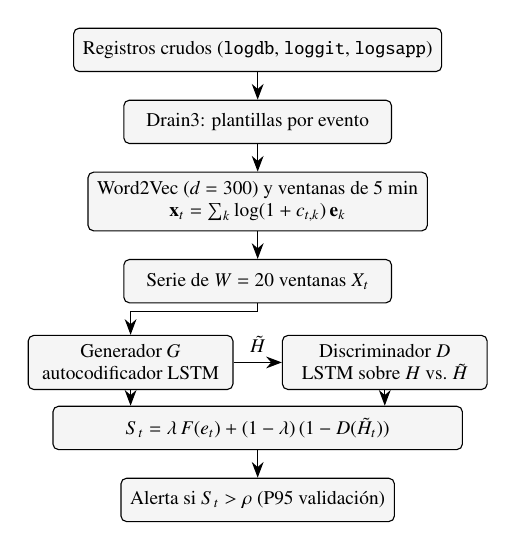
\begin{tikzpicture}[font=\scriptsize, node distance=3.5mm,
  b/.style={draw, rounded corners=2pt, align=center, minimum width=34mm, minimum height=5.5mm, fill=gray!8},
  a/.style={-{Stealth[length=2mm]}}]
\node[b] (raw) {Registros crudos (\texttt{logdb}, \texttt{loggit}, \texttt{logsapp})};
\node[b, below=of raw] (drain) {Drain3: plantillas por evento};
\node[b, below=of drain] (w2v) {Word2Vec ($d=300$) y ventanas de 5 min\\ $\vect{x}_t=\sum_k \log(1+c_{t,k})\,\vect{e}_k$};
\node[b, below=of w2v] (seq) {Serie de $W=20$ ventanas $X_t$};
\node[b, below left=4mm and -14mm of seq, minimum width=26mm] (G) {Generador $G$\\ autocodificador LSTM};
\node[b, below right=4mm and -14mm of seq, minimum width=26mm] (D) {Discriminador $D$\\ LSTM sobre $H$ vs.\ $\tilde H$};
\node[b, below=13mm of seq, minimum width=52mm] (S) {$S_t=\lambda\,F(e_t)+(1-\lambda)\,(1-D(\tilde H_t))$};
\node[b, below=of S] (dec) {Alerta si $S_t>\rho$ (P95 validación)};
\draw[a] (raw)--(drain); \draw[a] (drain)--(w2v); \draw[a] (w2v)--(seq);
\draw[a] (seq.south)--++(0,-1mm)-|(G.north); \draw[a] (G.east)--node[above]{$\tilde H$}(D.west);
\draw[a] (G.south)--(G.south|-S.north); \draw[a] (D.south)--(D.south|-S.north); \draw[a] (S)--(dec);
\end{tikzpicture}
\end{document}
